%  Typ dokumentu - článek, prezentace aj.
\documentclass[english]{article}

%  Nastaví vstupní a výstupní kódování znaků (encoding) a lokalizace
\usepackage[T1]{fontenc}
\usepackage[utf8]{inputenc}
\usepackage[english,czech]{babel}
\usepackage{icomma}

%  Formát papíru a odsazení od jeho okrajů
\usepackage[letterpaper]{geometry}
\geometry{verbose,tmargin=1.5cm,bmargin=2cm,lmargin=2cm,rmargin=2cm}

%  Umožňuje pracovat s grafikou
\usepackage{graphicx}
\usepackage{bigstrut}
\usepackage{epstopdf}

%  Automaticky odsadí i první paragraf v každé sekci
\usepackage{indentfirst}

%  Umožňuje rozdělovat obsah na více sloupců
\usepackage{multicol}
\usepackage{booktabs}
\usepackage{pgffor}
\usepackage{wrapfig}

%  Umožňuje používat hypertextové odkazy, nastavuje jejich barvu a vlastnosti
\usepackage[unicode]{hyperref}
\hypersetup{
	colorlinks=true, citecolor=blue, filecolor=blue, linkcolor=blue,
	urlcolor=blue
}

%  Umožnění odstranění italiky u jednotek
\newcommand{\unit}[1]{~\mathrm{#1}}
\newcommand{\unitb}[1]{~\mathrm{[#1]}}
\newcommand{\unitbr}[1]{\qquad\mathrm{[#1]}}


%  Formátování stránek, empty = odstraní číslování
% \pagestyle{empty}

%  Řádkování
\linespread{1.2}

%  Lepší zobrazování matematiky (rozšíření sum o \limits atd.)
%  Umožní psát přes \mathbb{N/R/Q/..} množiny čísel
\everymath{\displaystyle}
\usepackage{amsmath, amsthm, amssymb, wasysym}

%  Velikost fontu matematických výrazů v dokumentu lze pro danou
% základního fontu dokumentu upravit pomocí:
% \DeclareMathSizes{X}{Y}{Z}{U} kde:
% X je velikost fontu v dokumentu, pro kterou se matematika upraví
% Y je standartní velikost fontu matematiky
% Z je velikost fontu zmenšených (vnořených výrazů)
% U je velikost fontu ještě více zmenšených (vnořených výrazů).
\DeclareMathSizes{10}{10.5}{9}{9}

%  Nastaví autora, název, datum, skupinu měření apod. 
%  (můj vlastní příkaz, umožní znovu-použití v dokumentu)
\newcommand{\Author}{David Roesel}
\newcommand{\Coauthor}{Schönfeldová, Vyšín}
\newcommand{\Institute}{FJFI ČVUT v Praze}
\newcommand{\Subject}{VAKUOVÁ FYZIKA A TECHNIKA}
\newcommand{\Group}{Pá 14:30}
\newcommand{\Kruh}{FE}
\newcommand{\Title}{Úloha \#3  \\Hledání netěsností}
\newcommand{\Date}{21.11.2014}

% Custom comands
\newcommand{\dd}{\mathrm{d}}
\newcommand{\dln}{\mathrm{ln}}
\newcommand{\ee}{\mathrm{e}}
\newcommand{\jelina}{Oooo, Jelina!}

% Začátek dokumentu - Formátování na výstup
\begin{document}

% Interní proměnné, možno zobrazovat u prezentací, používají se při
% generování pomocí \titlepage apod.
\author{\Author}
\title{\Title}
\date{\Date}

%  Lokalizace některých názvů do češtiny
\renewcommand{\figurename}{Obr.}
\renewcommand{\tablename}{Tab.}
\renewcommand{\refname}{Reference}

% --- Hlavička dokumentu -----------------------------------------------

\setlength{\parindent}{0cm}
\begin{multicols}{2}
\textbf{\Subject \\
        \Institute \\[0.1cm]
%\large  \Title \\[0.5cm]
\Title \\[0.5cm]
}
\begin{tabular}{rlrl}
\large Datum měření: & \Date & \large Skupina: & \Group \\
\large Jméno: & \Author & \large Kroužek:  & \Kruh\\
\large Spolupracovali: & \Coauthor &\large Klasifikace:\\
\end{tabular}

\begin{flushright}

\includegraphics[scale=0.28]{../../_meta/fjfi_standart.pdf}
\hspace{0.2cm}

\includegraphics[scale=0.28]{../../_meta/cvut_standart.pdf}
\end{flushright}
\end{multicols}
\hrule
\vspace{0.5cm}

% ----------------------------------------------------------------------


% --- Tělo dokumentu ---------------------------------------------------
\setlength{\parindent}{0.5cm}

\section{Pracovní úkoly}
\begin{enumerate}
	\item Najděte netěsnost na skleněné trubici pomocí vtahování výboje vakuové zkoušečky.
	\item Ověřte změny zabarvení výboje ve skleněné trubici při ofukování netěsnosti heliem a při přikládání tamponu smočeného v lihu, isopropylalkoholu a acetonu k netěsnosti.
	\item Ověřte, že přivedení helia nebo par lihu, isopropylalkoholu a acetonu k netěsnosti (lehce pootevřený jehlový ventil) změní údaj tepelného vakuometru. Vysvětlete.
	\item Ověřte funkci halogenového hledače netěsností přikládáním tamponu, navlhčeného perchlorethylenem, k lehce otevřenému jehlovému ventilu. Vysvětlete.
	\item Seznamte se s heliovým hledačem netěsností. Seznamte se s duplikátem analyzační komůrky.
	\item Změřte indukci magnetického pole permanentního magnetu He-hledače. Z rozměrů uspořádání v komůrce a zjištěné hodnoty magnetického pole určete napětí, jímž musí být urychleny ionty helia, aby byl detekovaný jejich signál.
\end{enumerate}

\section{Úvod}
	Důležitou součástí práce s vakuovými aparaturami je bohužel hledání netěsností. Jejich vinou se zvyšuje mezní tlak, kterého je daná aparatura schopna dosáhnout, a snižuje se čerpací rychlost. Chceme-li získat dostatečně dobré vakuum, je třeba se netěsnostem věnovat a pokusit se je po nalezení odstranit.

%\begin{wrapfigure}{r}{0.5\textwidth}
%			\centering
%			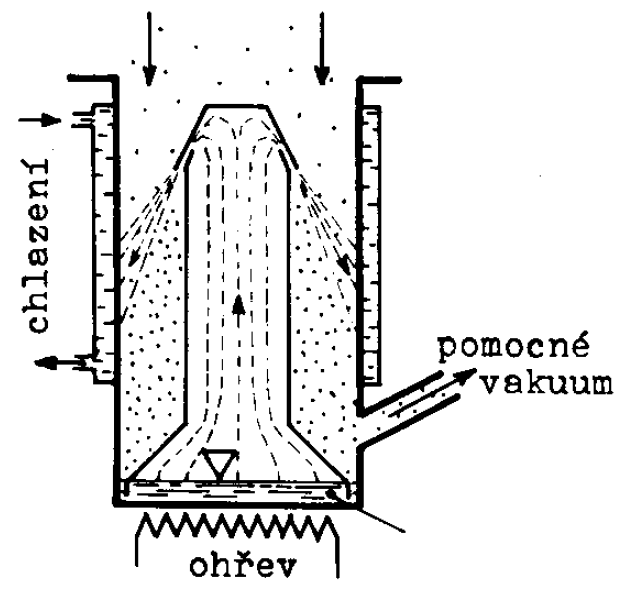
\includegraphics[width=5cm]{../att/difu_schema.png}
%			\caption{Schéma difusní vývěvy (převzato z \cite{bib:praskripta}).}
%			\label{fig:schema_dif}
%\end{wrapfigure}

\section{Vypracování}
	\subsection{Teoretický úvod}
		\subsubsection{Způsoby hledání netěsností}
			Netěsnosti můžeme v aparatuře hledat mnoha způsoby. Jedním z nich je využití vysokofrekvenční vakuové zkoušečky a vtahování jejího výboje. Je-li v materiálu (v našem řípadě ve skle) netěsnost, dojde ke vtáhnutí výboje do aparatury skrze ni a i při malém vychýlení zkoušečky se výboj stále váže do stejného místa.
			
			Dalším způsobem hledání netěsností může být využití různých barev výbojů v různých plynech či parách kapalin. Místa podezřelá z netěsnosti můžeme ofukovat například heliem či potírat kapalinami jako je líh, perchlorethylen nebo isopropylalkohol. Vnikne-li netěsností látka do aparatury, pozorujeme změnu barvy výboje. 
			
			Další vlastností různých plynů, kterou můžeme využít pro hledání netěsností, je jejich rozdílná tepelná vodivost vzhledem ke vzduchu. Zvýší-li se koncentrace těchto plynů v aparatuře, změní se údaj na tepelném manometru. Používáme-li ionizační manometry, uplatňují se různé ionizační účinné průřezy.
		
			Další metodou, kterou budeme studovat, je hledání pomocí halogenového hledače netěsností. Ten je založen na závislosti emise iontů alkalických kovů z horké platinové anody na přítomnosti halových prvků. 
			
			Nejpřesnější metodou, kterou si však prakticky nevyzkoušíme, je přímé měření obsahu testovaného plynu v aparatuře. Daný plyn má jasně definovanou hmotnost a jeho přítomnost se tak dá sledovat zjednodušeným hmotnostním spektrometrem, což je snazší pro lehčí plyny - nejčastěji používaným je helium. Heliový hledač je v principu samostatná vakuová komora, ve které se ionizuje zbytkový plyn, v němž se ionizují také ionty $\mathrm{He^+}$ a separují se. Následně se měří množství těchto iontů za ofukování netěsnosti heliem. Při průniku helia netěsností tedy pozorujeme nárůst výskytu těchto iontů. Na to, aby heliový hledač fungoval, musí být v komoře dostatečné vysoké vakuum. Vyčerpává se tedy nejprve rotační vývěvou a následně i vývěvou difusní. Dokud není chlazen lapač olejových par, nesmí se otevřít ventil spojující difusní vývěvu s analyzační komorou.  
			
		\subsubsection{Nabitá částice v homogenním magnetickém poli}
			Mějme částici o náboji $q$, která se pohybuje rychlostí $\vec{v}$ v homogenním čistě magnetickém poli o magnetické indukci $\vec{B}$, kde působí magnetická síla $\vec{F_m}$ o velikosti a směru
			\begin{equation}
				\vec{F_m} = q\vec{v}\times\vec{B}
			\end{equation}
			a jsou-li vektory $\vec{v}$ a $\vec{B}$ vzájemně kolmé, pak je k nim kolmý i vektor $\vec{F_m}$. Pro velikost magnetické síly potom bude platit
			\begin{equation}
				F_m=qvB,
			\end{equation}
			a tím pádem bude zakřivovat dráhu náboje. Nabitá částice se pak bude pohybovat po trajektorii opisující kruh o poloměru $r$. Při takovémto pohybu bude na částici působit dostředivá síla, jejíž velikost můžeme určit následovně:
			\begin{equation}
				F_d=\frac{mv^2}{r}
			\end{equation}
			a která bude mířit do středu kružnice. Vzhledem k tomu, že jsou velikosti sil $F_m$ a $F_d$ stejné, bude platit
			\begin{equation}
			F_m=qvB=\frac{mv^2}{r}=F_d.
			\label{eq:1_qvB}
			\end{equation}
			Počítáme-li s urychlovacím napětím $U$, bude mít díky němu nabitá částice energii $qU$, která se celá přemění na energii kinetickou. Platit tedy bude vztah
			\begin{equation}
				qU=\frac{mv^2}{2}.
			\label{eq:2_qU}
			\end{equation}
			
	\subsection{Postup měření}
		\subsubsection{Detekování netěsnosti pomocí vysokofrekvenční vakuové zkoušečky}
			Aparaturu jsme sestavili dle schématu na Obr.~\ref{fig:s_1} a za vlnovec jsme zařadili skleněnou trubici, která měla záhyb a na druhém konci byla zatavená. Zapnuli jsme rotační vývěvu a otevřením ventilu V1 jsme aparaturu vyčerpali. Následně jsme si vyzkoušeli, jak funguje vysokofrekvenční vakuová zkoušečka, kterou jsme přikládali k místům podél skleněné trubice a hledali možné netěsnosti. Nalezená místa jsme si pečlivě zaznamenali. 
		
		\subsubsection{Změna zbarvení výboje v závislosti na prostředí}
			Na tuto netěsnost jsme následně vyzkoušeli i další metodu hledání, tedy ofukování netěsnosti plynem, který mění barvu doutnavého výboje uvnitř v trubici. To jsme zkoušeli pomocí helia. Netěsnost jsme dále potírali také benzinem s lihem, perchlorethylenem a isopropylalkoholem. Při různých plynech jsme pozorovali různé barvy a naše pozorování jsme zaznamenávali.
		
		\subsubsection{Změna tepelné vodivosti v závislosti na prostředí}
			Na toto měření bylo třeba přestavit aparaturu do sestavení na Obr.~\ref{fig:s_2}. Jako recipient teď sloužila křížová nádoba, ke které byl připojen Piraniho tepelný manometr. Recipient jsme vyčerpali pomocí RV a mírně jsme pootevřeli jehlový ventil v recipientu, tak abychom jím mohli simulovat netěsnost. Na jehlový ventil jsme vyzkoušeli helium i všechny kapaliny z předchozího pokusu a sledovali jsme změnu ukazatele na tepelném manometru.

\begin{figure}[h!]
\centering
\begin{minipage}[t]{.40\textwidth}
\centering
				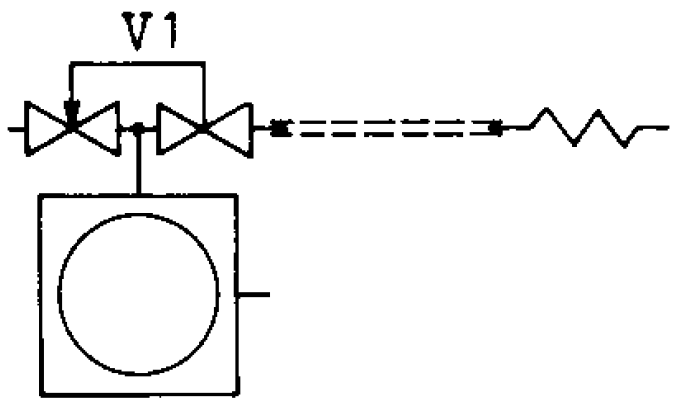
\includegraphics[scale=0.33]{../att/schema_vtahovani}
				\caption{Schéma sestavy pro zkoušky vtahování výboje do netěsnosti a barvení výboje při natékání různých látek - převzato z \cite{bib:praskripta}.}
				\label{fig:s_1}
\end{minipage}%
\hfill
\begin{minipage}[t]{.50\textwidth}
\centering
				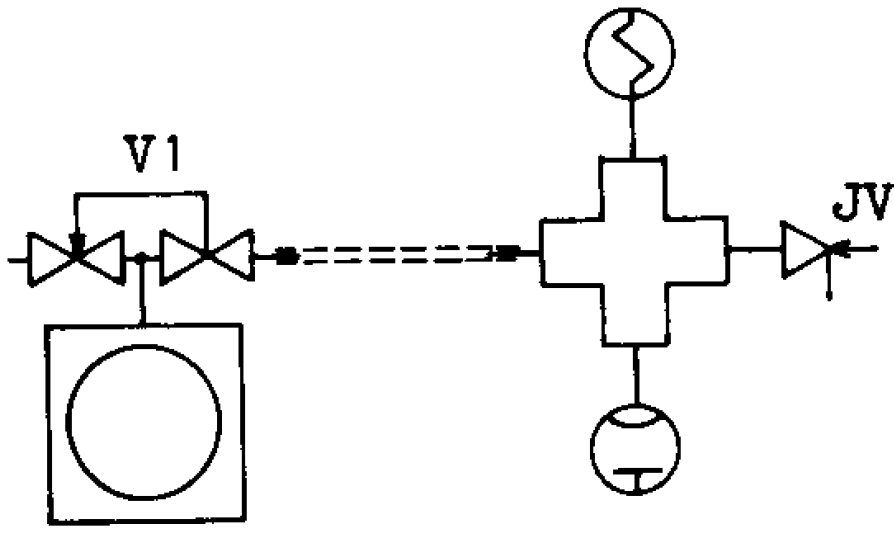
\includegraphics[scale=0.31]{../att/schema_tepelny}
				\caption{Schéma sestavy pro hledání netěsnosti pomocí Piraniho manometru a pomocí halogenového hledače - převzato z \cite{bib:praskripta}.}
				\label{fig:s_2}
\end{minipage}
\end{figure}
			
		\subsubsection{Halogenový hledač netěsností}
			\begin{wrapfigure}{r}{0.5\textwidth}
						\centering
						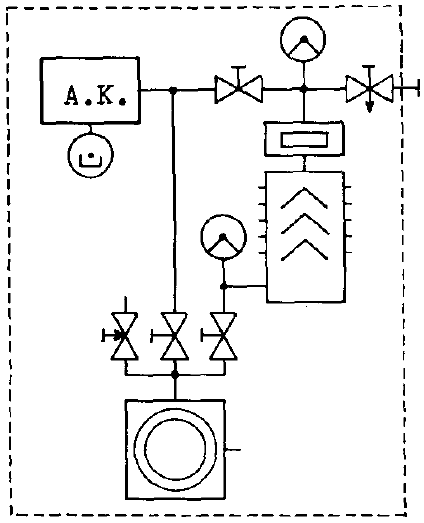
\includegraphics[width=5.5cm]{../att/schema_he}
						\caption{Vakuové schema heliového hledače netěsností, AK - analyzační komora - převzato z \cite{bib:praskripta}.}
						\label{fig:s_3}
						\vspace{-0.3cm}
			\end{wrapfigure}
			
			Aparaturu nebylo třeba přestavovat. Recipient již byl vyčerpán RV a po ustálení tlaku jsme pootevřeli jehlový ventil. Zapnuli jsme halogenový hledač netěsností a nastavili ho tak, aby byla ručička někde mírně pod polovinou stupnice - tedy aby měla místo nad i pod sebou. Vzhledem k očekávanému stoupání ručičky jsme později nulovali ručičku níže. 
			
			K simulované netěsnosti jsme následně pinzetou přikládali tampon navlhčený perchlorethylenem a pozorovali změny na halogenovém hledači. Tuto metodu jsme také využili k hledání dalších netěsností na aparatuře.
	
		\subsubsection{Heliový hledač netěsností}
					
			Prostudovali jsme heliový hledač netěsností i duplikát analyzační komory. Na duplikátu jsme změřili posuvným měřítkem průměr kružnice, kterou opisují urychlené ionty helia. Dále jsme změřili magnetickou indukci permanentního magnetu v heliovém hledači. 
			
	\subsection{Naměřené hodnoty}
		\subsubsection{Detekování netěsnosti pomocí vysokofrekvenční vakuové zkoušečky}
			Při hledání netěsnosí pomocí vysokofrekvenční vakuové zkoušečky jsme jednu nalezli přímo na konci skleněné trubice, kde byla zatavená. Výboj ze zkoušečky v relativně velkém okolí netěsnosti směřoval přesně do ní, jak je vidět na Obr.~\ref{fig:f_vyboj}. 
			
			\begin{figure} %{r}{0.5\textwidth}
						\centering
						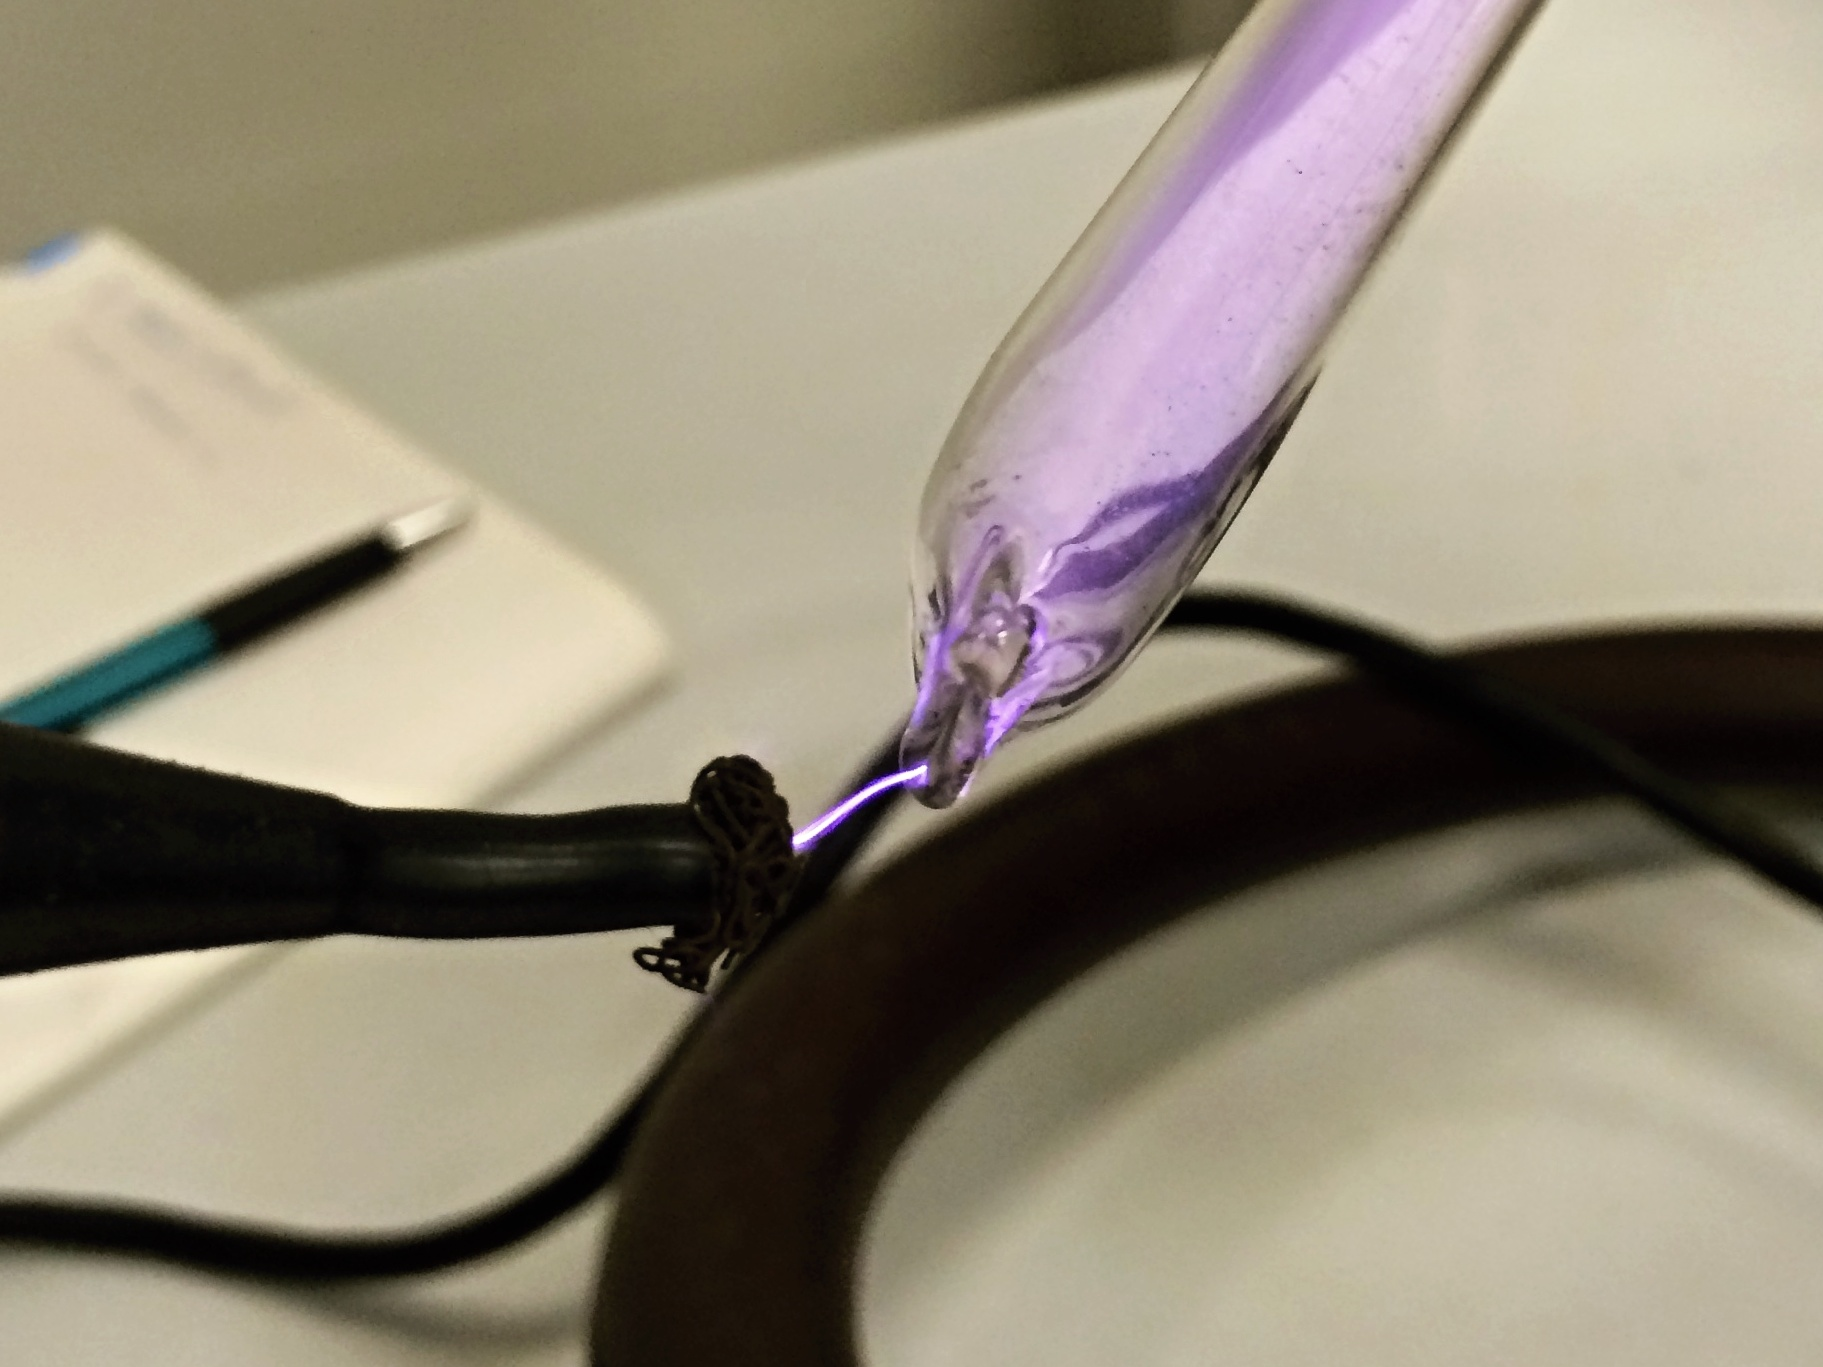
\includegraphics[width=8.5cm]{../att/vyboj}
						\caption{Pozorovaný výboj tekoucí do nalezené netěsnosti (vlastní tvorba).}
						\label{fig:f_vyboj}
			\end{figure}
		
		\subsubsection{Změna zbarvení výboje v závislosti na prostředí}
			Doutnavý výboj uvnitř skleněné trubice barvu neměnil v závislosti na prostředí příliš, ale to, co jsme pozorovali, je zaneseno do Tab.~\ref{tab:barvy}.
			
% Table generated by Excel2LaTeX from sheet 'List1'
\begin{table}[htbp]
  \centering
    \begin{tabular}{|r|r|}
    \hline
    \textbf{přivedená látka} & \textbf{barva výboje} \bigstrut\\
    \hline
    perchlorethylen & tmavší růžová \bigstrut\\
    \hline
    helium & světle modrá \bigstrut\\
    \hline
    isopropylalkohol & světlejší fialová \bigstrut\\
    \hline
    líh s benzínem & zmizení výboje \bigstrut\\
    \hline
    \end{tabular}%
  \caption{Pozorované jevy při studování výboje ze zkoušečky za přivádění různých látek k netěsnosti.}
  \label{tab:barvy}%
\end{table}%
			
		
		\subsubsection{Změna tepelné vodivosti v závislosti na prostředí}
			Pokaždé, když jsme jehlový ventil ofoukli heliem nebo potřeli některou z kapalin, údaj na manometru stoupl, avšak ne o takovou hodnotu, aby se daly přesněji porovnávat. Pozorované jevy jsou tedy zaneseny do Tab.~\ref{tab:tepel}, ale jedná se spíše o zběžné relativní porovnání.
		
% Table generated by Excel2LaTeX from sheet 'List1'
\begin{table}[htbp]
  \centering
    \begin{tabular}{|r|r|}
    \hline
    \textbf{přivedená látka} & \textbf{pozorovaný jev} \bigstrut\\
    \hline
    helium & mírné zvýšení \bigstrut\\
    \hline
    isopropylalkohol & zvýšení na 100 Pa \bigstrut\\
    \hline
    líh s benzínem & zvýšení na 80 Pa \bigstrut\\
    \hline
    perchlorethylen & zvýšení na 50 Pa \bigstrut\\
    \hline
    \end{tabular}%
  
  \caption{Tabulka pozorovaných tlakových změn za přivádění různých látek k netěsnosti.}
  \label{tab:tepel}%
\end{table}%
		

		\subsubsection{Halogenový hledač netěsností}
			V momentu, kdy jsme k netěsnosti přiložili tampon s perchlorethylenem, ručička na hledači vyskočila prudce nahoru mimo stupnici ve všech případech. Pomocí této metody jsme odhalili také další netěsnosti na aparatuře, převážně v blízkosti těsnění mezi recipientem a senzorem Piraniho manometru a spoje RV s recipientem.
		
		\subsubsection{Heliový hledač netěsností}
			Poloměr kruhové trajektorie, po které létají ionty helia, jsme určili pomocí posuvného měřítka s chybou poloviny nejmenšího dílku jako 
			\begin{equation}
				r = (40,0\pm0,5)\unit{mm}.
			\end{equation}
			
			Velikost magnetické indukce v analyzátoru jsme změřili Teslametrem s odhadnutou chybou jako 
			\begin{equation}
				B = (143\pm1)\unit{mT}.
			\end{equation}
			Budeme-li poměr $q$ a $m$ pro helium uvažovat dle \cite{bib:constants}
			\begin{equation}
				\frac{q}{m}=2,41\cdot 10^7\unit{C/kg},
			\end{equation}
			můžeme urychlovací napětí iontů $\mathrm{He^{+}}$ pomocí vztahů (\ref{eq:1_qvB}) a (\ref{eq:2_qU}) určit s chybou podle (\ref{eq:chyba_neprime_mereni}) jako
			\begin{equation}
				U = (390\pm10)\unit{V}.
			\end{equation}
			
	\subsection{Diskuse}
    	
		\subsubsection{Detekování netěsnosti pomocí vysokofrekvenční vakuové zkoušečky}
			Pomocí vysokofrekvenční vakuové zkoušečky jsme úspěšně detekovali netěsnost na konci skleněné trubice, kde byla zatavená. Bylo evidentní, že je výboj vtahován spodní částí konce i při mírném vzdálení zkoušečky od netěsnosti. Ačkoliv jsme vysokofrekvenční zkoušečkou otestovali i zbytek skleněné trubice, další netěsnost jsme nenašli. Očekávali bychom, že najdeme další netěsnost v ohybu skleněné trubice. Pokud tam ale nějaké netěsnosti byly, pak musely být pod detekčním limitem vakuové zkoušečky.
			
		\subsubsection{Změna zbarvení výboje v závislosti na prostředí}
			Netěsnost jsme potírali různými sloučeninami, ofukovali heliem a u některých z nich jsme úspěšně pozorovali změnu barvy doutnavého výboje v závislosti na prostředí uvnitř skleněné trubice. Zajímavostí při tomto pokusu bylo, že při potření netěsnosti lihem s benzínem výboj místo změny barvy úplně zmizel. Tuto skutečnost můžeme přisuzovat tomu, že kapalina na netěsnosti zamrzla a zabránila tím vniku dalšího vzduchu do recipientu. Druhou možností je, že výboj měl šedobílou barvu a my jsme ji nebyli schopni rozeznat. Nutno je také poznamenat, že vnímání barev je velice subjektivní a zjištěné hodnoty tedy velice závisí na tom, kdo ze skupiny je pozoroval.
		
		\subsubsection{Změna tepelné vodivosti v závislosti na prostředí}
		 	Při přikládání lihu s benzínem, isopropylalkoholu a perchlorethylenu jsme pozorovali nárůst tlaku na tepelném manometru. Tento nárůst je způsoben tím, že páry daných sloučenin mají vyšší tepelnou vodivost než vzduch a tím, že rychleji vtékají do aparatury. Pozorovaná míra zvýšení tlaku byla závislá na tom, jak dobře se nám podařilo trefit netěsnost a jak moc byl pootevřený jehlový ventil, kterým jsme netěsnost simulovali. Kdybychom věnovali dost času hledání lepší polohy tamponu se sloučeninami, povedlo by se nám možná dosáhnout i zvýšení o více než 100 Pa.
		
		\subsubsection{Halogenový hledač netěsností}
			Při měření halogenovým hledačem jsme přikládali k netěsnostem perchlorethylen, ale nemůžeme přesně stanovit, o kolik se zvýšil tlak, jelikož při každém přiložení ukazatel vylétl ze stupnice. To bylo zapříčiněno zvýšenou emisí alkalických kovů z horké anody způsobené přítomností chloru, který patří mezi halogeny, v perchlorethylenu. Ač nám tato metoda neumožňovala zjistit konkrétní hodnoty nárůstu tlaku, využili jsme ji k nalezení dalších dvou netěsností na aparatuře, které nám do té doby unikly. Obě z nich byly v blízkosti gumových těsnění, kde jsme jejich přítomnost očekávali.
						
		\subsubsection{Heliový hledač netěsností}
			Heliový hledač jsme si bohužel neměli možnost vyzkoušet v akci. Prozkoumali jsme však důkladně jeho konstrukci a popsali ji v teoretickém úvodu. Provedli jsme výpočty pro určení urychlovacího napětí iontů helia. Je však nutné poznamenat, že tento výpočet byl proveden za předpokladu homogenního magnetického pole uvnitř heliového hledače a to se nám při měření jako homogenní nejevilo. Snažili jsme se teslametrem dostat na co nejlepší místo, ale naměřenou hodnotu musíme stále brát s jistou rezervou.
			
			V případě, že bychom měli heliový hledač zprovozněný, nastal by stejný problém, jako s heliem nastával během předchozích experimentů. Stávalo se nám totiž, že se intenzita pozorovaných jevů dramaticky měnila v závislosti na nasměrování koncovky hadice, vedoucí z heliového balónku. I proto předpokládáme, že bychom museli pro přesnější měření foukat na hledané netěsnosti správným směrem.

\section{Závěr}
	Našli jsme netěsnost na konci skleněné trubice pomocí vtahování výboje vakuové zkoušečky.
	
	Ověřili jsme změny zabarvení výboje ve skleněné trubici při ofukování netěsnosti heliem a při přikládání tamponu smočeného v lihu, isopropylalkoholu a perchlorethylenu k netěsnosti. 
	
	Ověřili jsme, že přivedení helia nebo par lihu, isopropylalkoholu a perchlorethylenu k netěsnosti (lehce pootevřený jehlový ventil) změní údaj tepelného vakuometru. Tento jev jsme vysvětlili.
	
	Ověřili jsme funkci halogenového hledače netěsností a seznámili jsme se s duplikátem analyzační komůrky.
	
	Změřili jsme indukci magnetického pole permanentního magnetu He-hledače. Z rozměrů uspořádání v komůrce a zjištěné hodnoty magnetického pole jsme určili napětí, jímž musí být urychleny ionty helia, aby byl detekován jejich signál, jako $U = (390\pm10)\unit{V}$.
	
\section {Použitá literatura}
% --- Literatura a reference -------------------------------------------
\begingroup
\renewcommand{\section}[2]{}

\begin{thebibliography}{9}

\bibitem{bib:chyby} Kolektiv KF, \emph{Chyby měření} [Online], [cit. \today] \newline http://praktikum.fjfi.cvut.cz/documents/chybynav/chyby-o.pdf

\bibitem{bib:praskripta}Král, J.: \emph{Cvičení z vakuové techniky},
Vydavatelství ČVUT, Praha, 1996

%\bibitem{bib:tlak}ČHMÚ: \emph{Aktuální informace o počasí na území České republiky}, {[}online{]}, {[}cit. \today{]},\newline http://pr-asv.chmi.cz/synopy-map/pocasisp.php?ukazatel=stanice\&pozadi=\&pozadi=mapareg\&graf=ano

\bibitem{bib:constants}NIST Physical Measurement Laboratory: \emph{Fundamental Physical Constants} [Online], [cit \today] \newline http://physics.nist.gov/cgi-bin/cuu/Category?view=html\&Atomic+and+nuclear.x=114\&Atomic+and+nuclear.y=11
 

\end{thebibliography}
\endgroup
% ----------------------------------------------------------------------
\setcounter{equation}{0}
\numberwithin{equation}{section}

\clearpage
\part*{Přílohy}

%\section{Domácí příprava}
%	Domácí příprava je přiložena k protokolu.
%\clearpage
\section{Statistické zpracování dat}
	Pro statistické zpracování využíváme aritmetického průměru:
	\begin{equation} \label{eq:aritmeticky_prumer}
	\overline{x} = \frac{1}{n}\sum\limits_{i=1}^{n}x_i,
	\end{equation}

%	jehož směrodatnou odchylku spočítáme jako 
%	\begin{equation} \label{eq:smodch_aritmetickeho_prumeru}
%	\sigma_0 = \sqrt{\frac{1}{n} \sum\limits_{i=1}^{n}\left( x_i - \overline{x} \right)^2 },
%	\end{equation}
%	
%	kde $ x_i $ jsou jednotlivé naměřené hodnoty, $ n $ je počet měření, $ \overline{x} $ aritmetický průměr a $ \sigma_0 $ jeho chyba \cite{bib:chyby}.
	
	
	jehož chybu spočítáme jako 
	\begin{equation} \label{eq:chyba_aritmetickeho_prumeru}
	\sigma_0 = \sqrt{\frac{1}{n(n-1)} \sum\limits_{i=1}^{n}\left( x_i - \overline{x} \right)^2 },
	\end{equation}
	
	kde $ x_i $ jsou jednotlivé naměřené hodnoty, $ n $ je počet měření, $ \overline{x} $ aritmetický průměr a $ \sigma_0 $ jeho chyba \cite{bib:chyby}.
%	
Při nepřímém měření počítáme hodnotu s chybou dle následujících vztahů:
	\begin{equation}
	u = f(x, y, z, \ldots),
	\end{equation}
	\begin{displaymath}
	x = (\overline{x} \pm \sigma_x), \qquad
	y = (\overline{y} \pm \sigma_y), \qquad
	z = (\overline{z} \pm \sigma_z), \qquad
	\ldots,
	\end{displaymath}
	
	kde $ u $ je veličina, kterou určujeme nepřímo z měřených veličin $ x, y, z, \ldots $ 
	
	Pak
	\begin{displaymath}
	\overline{u} = f(\overline{x}, \overline{y}, \overline{z}, \ldots),
	\end{displaymath}
	\begin{equation}\label{eq:chyba_neprime_mereni}
	\sigma_u = \sqrt{\left( \frac{\partial f}{\partial x} \right)^2 \sigma^2_x + \left( \frac{\partial f}{\partial y} \right)^2 \sigma^2_y + \left( \frac{\partial f}{\partial z} \right)^2 \sigma^2_z + \ldots},
	\end{equation}
	\begin{displaymath}
	u = (\overline{u} \pm \sigma_ u).
	\end{displaymath}
%%	
%V případě, že máme několik různě přesných měření stejné veličiny, používáme vztah pro vážený průměr:
%	\begin{equation} 
%	\overline{x}=\frac{\sum\limits_{i=1}^{n}p_{i}x_{i}}{\sum\limits_{i=1}^{n}p_{i}},
%	\end{equation}
%	
%	kde $\overline{x}$ je vážený průměr, $x_{i}$ jsou jednotlivá měření a pro $p_{i}$ platí
%	 
%	\begin{equation}
%	p_{i}=\frac{1}{\sigma_{i}^{2}},
%	\end{equation}
%	
%	kde $\sigma_{i}$ jsou jednotlivé chyby daných měření.
%	 
%	Celkovou chybu tedy vypočítáme ze vztahu
%	\begin{equation} \label{eq:vazeny_prumer}
%	\sigma_{0}=\sqrt{\frac{1}{\sum\limits_{i=1}^{n}p_{i}}}.
%	\end{equation}
%
%\subsubsection{Metoda nejmenších čtverců}
%Snažíme-li se metodou nejmenších čtverců proložit data lineární závislostí $Y_i = ax_i+b$, dosazujeme hodnoty $x_i, y_i$ a snažíme se najít parametry $a$ a $b$ tak, aby byl součet všech kvadratických odchylek $\Delta Y_i^2$ minimální. Toho dosáhneme pomocí následujících vzorců \cite{bib:ctverce} :
%\begin{equation}\label{eq:ctverce_a}
%		a = \frac{n\sum\limits_{i=1}^{n}{x_i y_i}  - \sum\limits_{i=1}^{n}{x_i}\sum\limits_{i=1}^{n}{y_i}}{n\sum\limits_{i=1}^{n}{x_i^2}  - \left(\sum\limits_{i=1}^{n}{x_i}\right)^2}, \qquad \qquad
%		\sigma_a = \sqrt{\frac{n\sum\limits_{i=1}^{n}{(y_i - Y_i)^2} }{(n-2)\left(\sum\limits_{i=1}^{n}{x_i^2}  - \left(\sum\limits_{i=1}^{n}{x_i}\right)^2\right)}},
%\end{equation}
%
%\begin{equation}\label{eq:ctverce_b}
%		b = \frac{\sum\limits_{i=1}^{n}{x_i^2} \sum\limits_{i=1}^{n}{y_i}  - \sum\limits_{i=1}^{n}{x_i}\sum\limits_{i=1}^{n}{x_i y_i}}{n\sum\limits_{i=1}^{n}{x_i^2}  - \left(\sum\limits_{i=1}^{n}{x_i}\right)^2}, \qquad \qquad
%		\sigma_b = \sqrt{\frac{\sum\limits_{i=1}^{n}{x_i^2}\sum\limits_{i=1}^{n}{(y_i - Y_i)^2} }{n(n-2)\left(\sum\limits_{i=1}^{n}{x_i^2}  - \left(\sum\limits_{i=1}^{n}{x_i}\right)^2\right)}}.
%\end{equation}
	
%\clearpage

%\catcode`\-=12 % HAX na enable cline v českym bable
%\subsection{Tabulky a grafy}

%\begin{figure}[h!]
%	\begin{center}
%		\vspace*{-0.5cm}
%		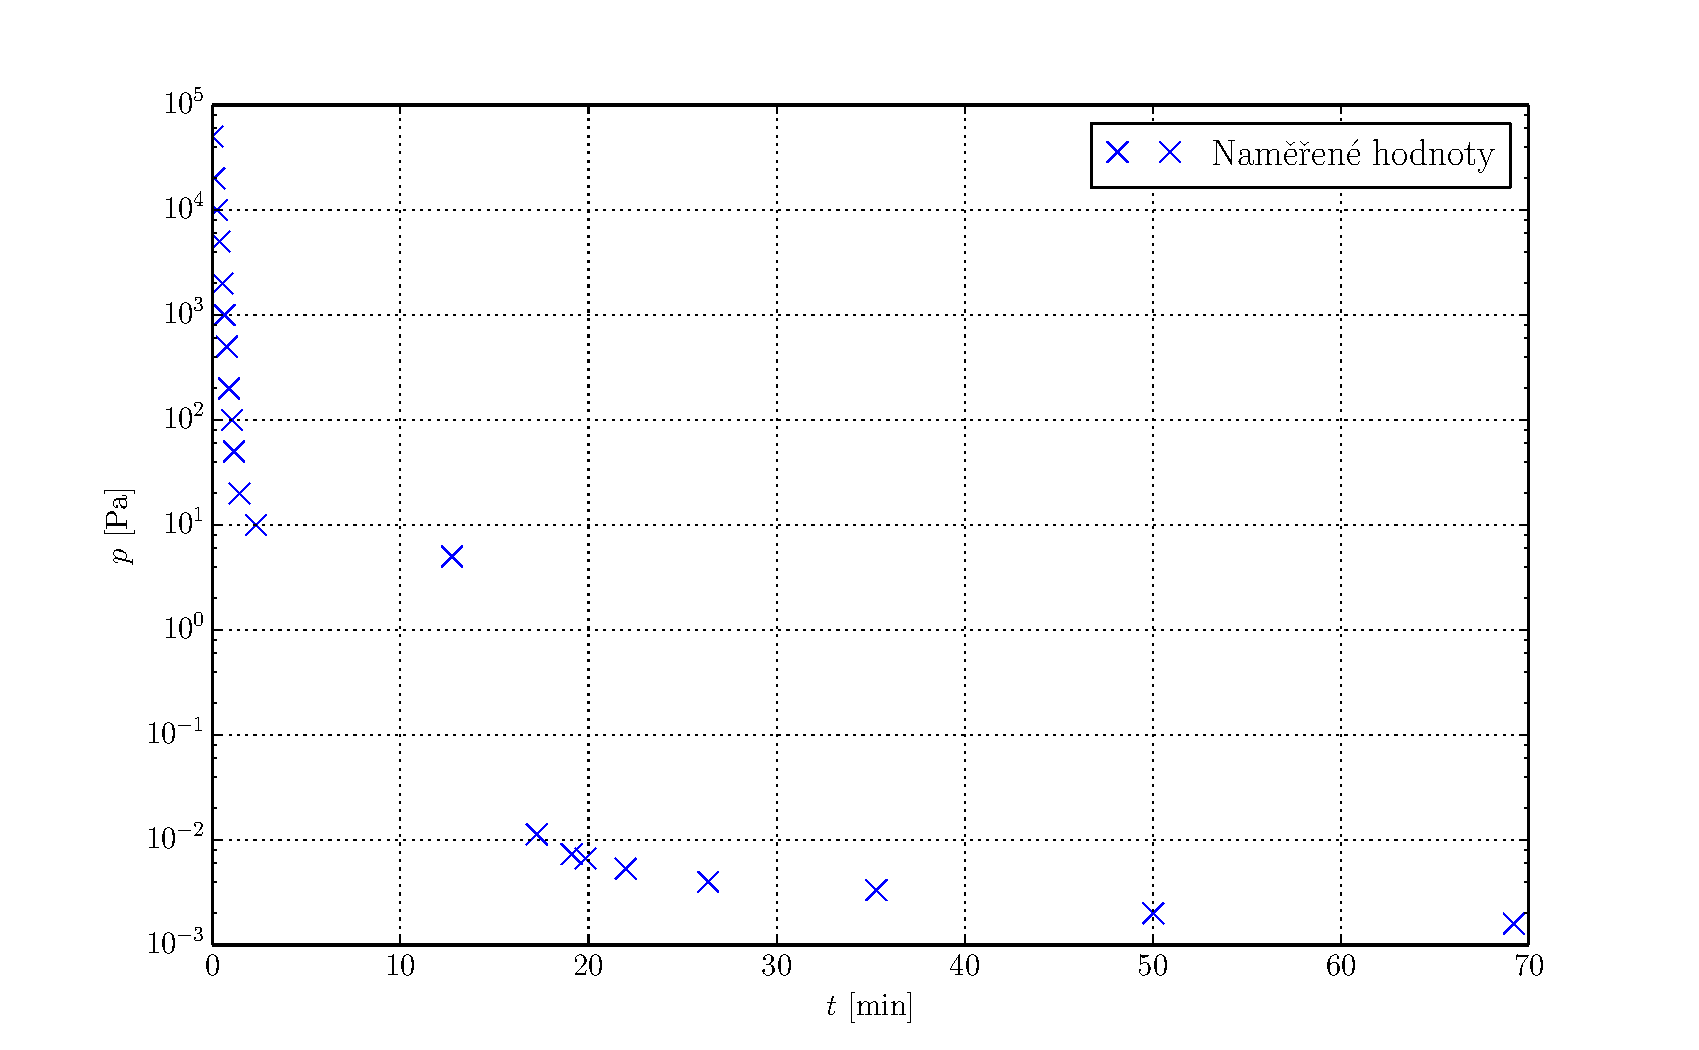
\includegraphics[width=\linewidth]{../plt/01_p.pdf}
%		\vspace*{-0,7cm}
%		\caption{Graf závislosti tlaku v recipientu $p$ na čase $t$. Difusní vývěvu jsme zapnuli zhruba ve 13. minutě. Osamocená hodnota kolem 11. minuty není chyba měření, viz diskuse.}
%		\label{fig:g_tlak}
%	\end{center}
%\end{figure}

%\clearpage
%\subsection{Schémata}
%	
%	\begin{figure}[h!]
%	\centering
%			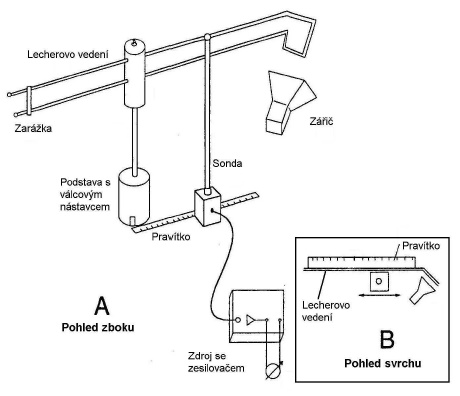
\includegraphics[width=13cm]{att/lecherovo_vedeni.jpg}
%			\caption{Experiment s Lecherovým vedením (převzato z  \cite{bib:zadani}). }
%			\label{fig:lecherovo_vlneni}
%	\end{figure}	
%	
%\clearpage
% --- Konec dokumentu --------------------------------------------------

\end{document}

